\documentclass[border=12pt]{standalone}
\usepackage{tikz}
\usetikzlibrary{shapes.geometric, arrows.meta, positioning, calc, fit, backgrounds}
\usepackage{fontspec}
\usepackage{amsmath}
\setmainfont{DejaVu Sans}

\begin{document}
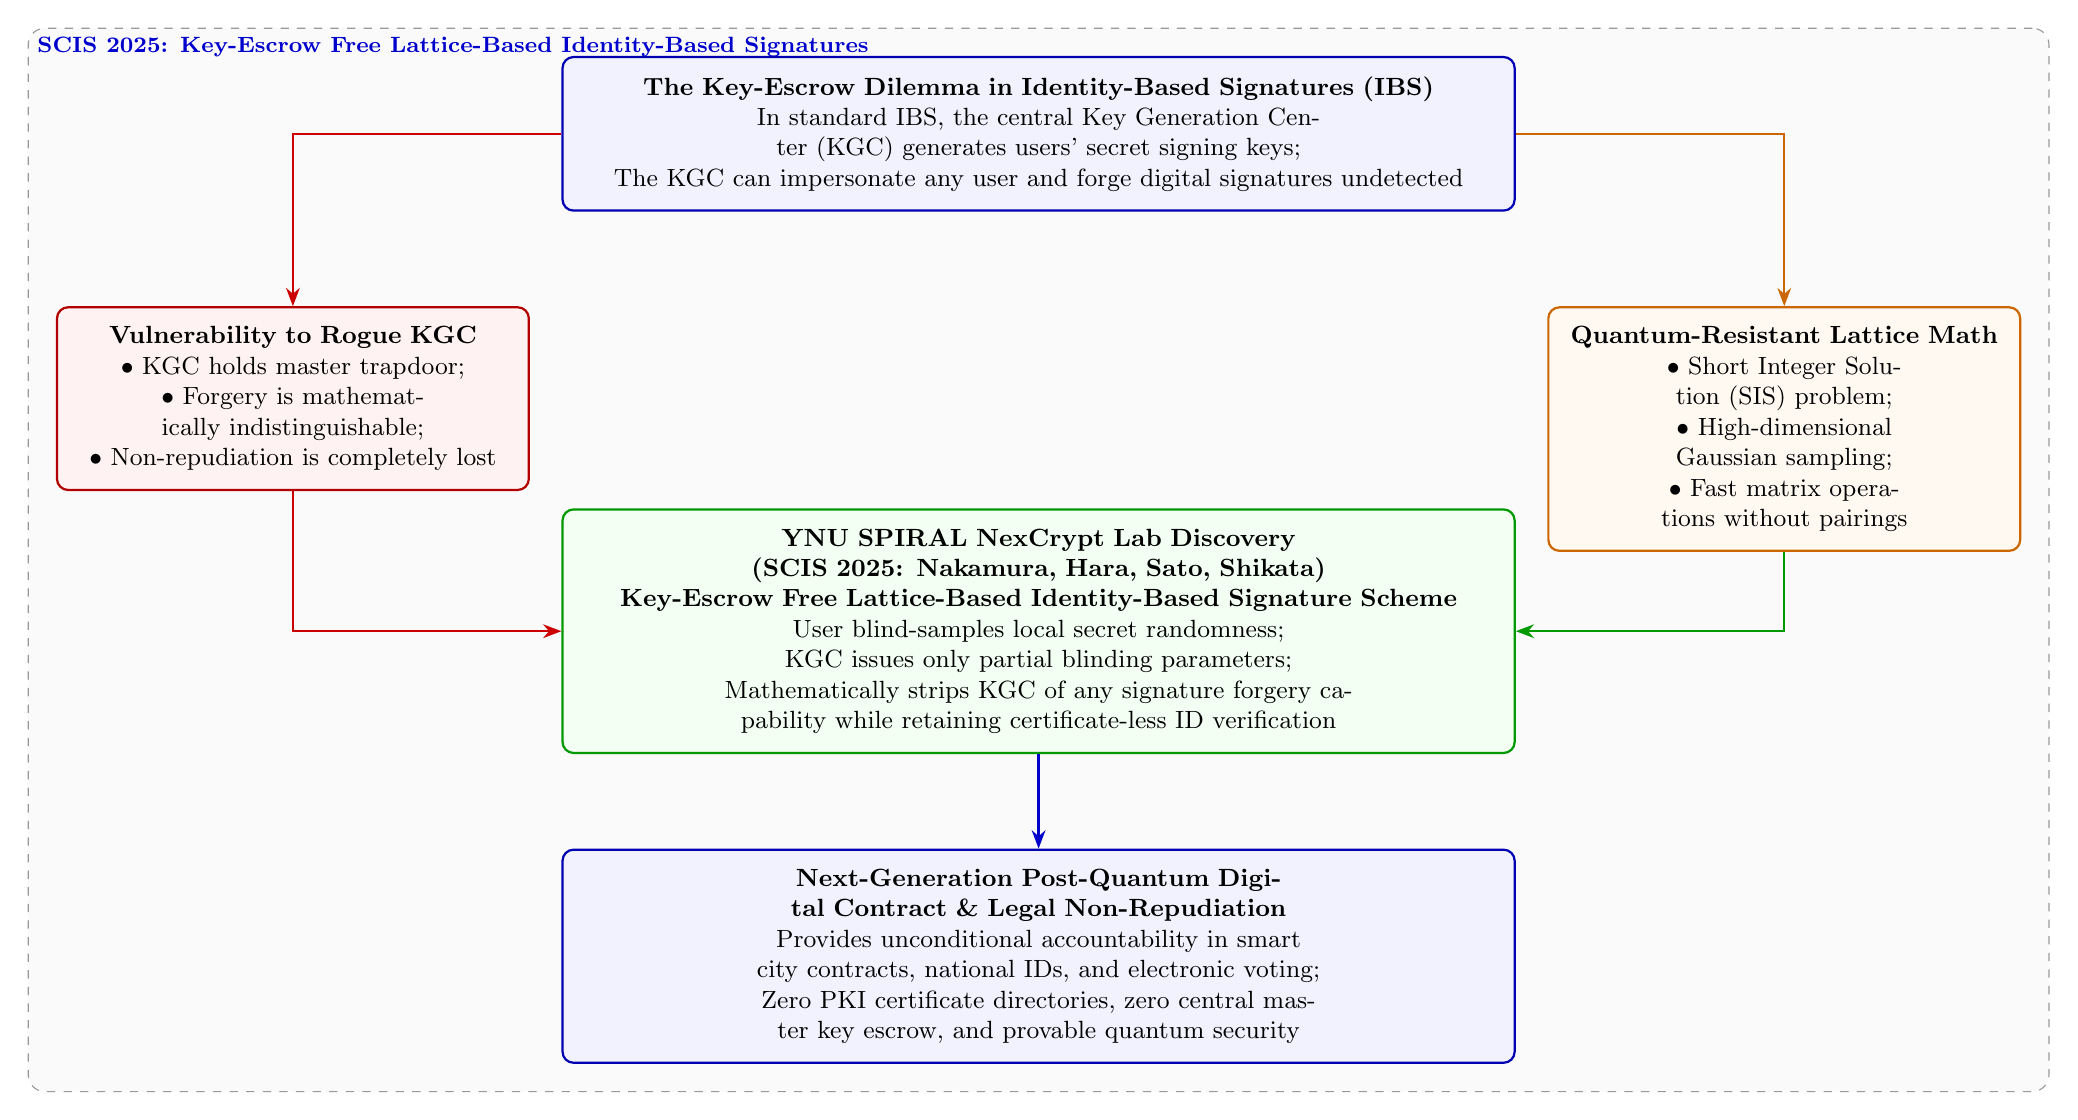
\begin{tikzpicture}[
    font=\small,
    >=Stealth,
    node distance=1.2cm,
    block/.style={rectangle, draw=blue!70!black, fill=blue!5, rounded corners=4pt, thick, align=center, inner sep=7pt},
    alertblock/.style={rectangle, draw=red!70!black, fill=red!5, rounded corners=4pt, thick, align=center, inner sep=7pt},
    greenblock/.style={rectangle, draw=green!60!black, fill=green!5, rounded corners=4pt, thick, align=center, inner sep=7pt},
    amberblock/.style={rectangle, draw=orange!80!black, fill=orange!5, rounded corners=4pt, thick, align=center, inner sep=7pt},
    groupbox/.style={draw=black!40, dashed, rounded corners=6pt, fill=black!2, inner sep=10pt}
]

    % Top: The Core Dilemma in Identity-Based Signatures
    \node[block, text width=11.6cm] (dilemma) {\textbf{The Key-Escrow Dilemma in Identity-Based Signatures (IBS)}\\In standard IBS, the central Key Generation Center (KGC) generates users' secret signing keys;\\The KGC can impersonate any user and forge digital signatures undetected};

    % Left: Traditional Traitors
    \node[alertblock, below left=1.2cm and 0.4cm of dilemma, text width=5.5cm] (escrow) {\textbf{Vulnerability to Rogue KGC}\\$\bullet$ KGC holds master trapdoor;\\$\bullet$ Forgery is mathematically indistinguishable;\\$\bullet$ Non-repudiation is completely lost};

    % Right: Lattice Hardness Under Post-Quantum
    \node[amberblock, below right=1.2cm and 0.4cm of dilemma, text width=5.5cm] (lattice) {\textbf{Quantum-Resistant Lattice Math}\\$\bullet$ Short Integer Solution (SIS) problem;\\$\bullet$ High-dimensional Gaussian sampling;\\$\bullet$ Fast matrix operations without pairings};

    \draw[->, thick, red!80!black] (dilemma) -| (escrow);
    \draw[->, thick, orange!80!black] (dilemma) -| (lattice);

    % Middle: YNU Breakthrough (SCIS 2025: Nakamura, Hara, Sato, Shikata)
    \node[greenblock, below=1.2cm of $(escrow)!0.5!(lattice)$, text width=11.6cm] (breakthrough) {\textbf{YNU SPIRAL NexCrypt Lab Discovery (SCIS 2025: Nakamura, Hara, Sato, Shikata)}\\\textbf{Key-Escrow Free Lattice-Based Identity-Based Signature Scheme}\\User blind-samples local secret randomness; KGC issues only partial blinding parameters;\\Mathematically strips KGC of any signature forgery capability while retaining certificate-less ID verification};

    \draw[->, thick, red!80!black] (escrow) |- (breakthrough);
    \draw[->, thick, green!60!black] (lattice) |- (breakthrough);

    % Bottom: Impact
    \node[block, below=1.2cm of breakthrough, text width=11.6cm] (impact) {\textbf{Next-Generation Post-Quantum Digital Contract \& Legal Non-Repudiation}\\Provides unconditional accountability in smart city contracts, national IDs, and electronic voting;\\Zero PKI certificate directories, zero central master key escrow, and provable quantum security};

    \draw[->, thick, blue!80!black] (breakthrough) -- (impact);

    \begin{scope}[on background layer]
        \node[groupbox, fit=(dilemma) (escrow) (lattice) (breakthrough) (impact), label={[anchor=north west, font=\footnotesize\bfseries, blue!80!black]north west:SCIS 2025: Key-Escrow Free Lattice-Based Identity-Based Signatures}] {};
    \end{scope}

\end{tikzpicture}
\end{document}
